\PassOptionsToPackage{unicode=true}{hyperref} % options for packages loaded elsewhere
\PassOptionsToPackage{hyphens}{url}
%
\documentclass[
]{article}
\usepackage{lmodern}
\usepackage{amssymb,amsmath}
\usepackage{ifxetex,ifluatex}
\ifnum 0\ifxetex 1\fi\ifluatex 1\fi=0 % if pdftex
  \usepackage[T1]{fontenc}
  \usepackage[utf8]{inputenc}
  \usepackage{textcomp} % provides euro and other symbols
\else % if luatex or xelatex
  \usepackage{unicode-math}
  \defaultfontfeatures{Scale=MatchLowercase}
  \defaultfontfeatures[\rmfamily]{Ligatures=TeX,Scale=1}
\fi
% use upquote if available, for straight quotes in verbatim environments
\IfFileExists{upquote.sty}{\usepackage{upquote}}{}
\IfFileExists{microtype.sty}{% use microtype if available
  \usepackage[]{microtype}
  \UseMicrotypeSet[protrusion]{basicmath} % disable protrusion for tt fonts
}{}
\makeatletter
\@ifundefined{KOMAClassName}{% if non-KOMA class
  \IfFileExists{parskip.sty}{%
    \usepackage{parskip}
  }{% else
    \setlength{\parindent}{0pt}
    \setlength{\parskip}{6pt plus 2pt minus 1pt}}
}{% if KOMA class
  \KOMAoptions{parskip=half}}
\makeatother
\usepackage{xcolor}
\IfFileExists{xurl.sty}{\usepackage{xurl}}{} % add URL line breaks if available
\IfFileExists{bookmark.sty}{\usepackage{bookmark}}{\usepackage{hyperref}}
\hypersetup{
  pdftitle={Wavelet Screaming on methyaltion},
  pdfauthor={William Denault},
  pdfborder={0 0 0},
  breaklinks=true}
\urlstyle{same}  % don't use monospace font for urls
\usepackage[margin=1in]{geometry}
\usepackage{color}
\usepackage{fancyvrb}
\newcommand{\VerbBar}{|}
\newcommand{\VERB}{\Verb[commandchars=\\\{\}]}
\DefineVerbatimEnvironment{Highlighting}{Verbatim}{commandchars=\\\{\}}
% Add ',fontsize=\small' for more characters per line
\usepackage{framed}
\definecolor{shadecolor}{RGB}{248,248,248}
\newenvironment{Shaded}{\begin{snugshade}}{\end{snugshade}}
\newcommand{\AlertTok}[1]{\textcolor[rgb]{0.94,0.16,0.16}{#1}}
\newcommand{\AnnotationTok}[1]{\textcolor[rgb]{0.56,0.35,0.01}{\textbf{\textit{#1}}}}
\newcommand{\AttributeTok}[1]{\textcolor[rgb]{0.77,0.63,0.00}{#1}}
\newcommand{\BaseNTok}[1]{\textcolor[rgb]{0.00,0.00,0.81}{#1}}
\newcommand{\BuiltInTok}[1]{#1}
\newcommand{\CharTok}[1]{\textcolor[rgb]{0.31,0.60,0.02}{#1}}
\newcommand{\CommentTok}[1]{\textcolor[rgb]{0.56,0.35,0.01}{\textit{#1}}}
\newcommand{\CommentVarTok}[1]{\textcolor[rgb]{0.56,0.35,0.01}{\textbf{\textit{#1}}}}
\newcommand{\ConstantTok}[1]{\textcolor[rgb]{0.00,0.00,0.00}{#1}}
\newcommand{\ControlFlowTok}[1]{\textcolor[rgb]{0.13,0.29,0.53}{\textbf{#1}}}
\newcommand{\DataTypeTok}[1]{\textcolor[rgb]{0.13,0.29,0.53}{#1}}
\newcommand{\DecValTok}[1]{\textcolor[rgb]{0.00,0.00,0.81}{#1}}
\newcommand{\DocumentationTok}[1]{\textcolor[rgb]{0.56,0.35,0.01}{\textbf{\textit{#1}}}}
\newcommand{\ErrorTok}[1]{\textcolor[rgb]{0.64,0.00,0.00}{\textbf{#1}}}
\newcommand{\ExtensionTok}[1]{#1}
\newcommand{\FloatTok}[1]{\textcolor[rgb]{0.00,0.00,0.81}{#1}}
\newcommand{\FunctionTok}[1]{\textcolor[rgb]{0.00,0.00,0.00}{#1}}
\newcommand{\ImportTok}[1]{#1}
\newcommand{\InformationTok}[1]{\textcolor[rgb]{0.56,0.35,0.01}{\textbf{\textit{#1}}}}
\newcommand{\KeywordTok}[1]{\textcolor[rgb]{0.13,0.29,0.53}{\textbf{#1}}}
\newcommand{\NormalTok}[1]{#1}
\newcommand{\OperatorTok}[1]{\textcolor[rgb]{0.81,0.36,0.00}{\textbf{#1}}}
\newcommand{\OtherTok}[1]{\textcolor[rgb]{0.56,0.35,0.01}{#1}}
\newcommand{\PreprocessorTok}[1]{\textcolor[rgb]{0.56,0.35,0.01}{\textit{#1}}}
\newcommand{\RegionMarkerTok}[1]{#1}
\newcommand{\SpecialCharTok}[1]{\textcolor[rgb]{0.00,0.00,0.00}{#1}}
\newcommand{\SpecialStringTok}[1]{\textcolor[rgb]{0.31,0.60,0.02}{#1}}
\newcommand{\StringTok}[1]{\textcolor[rgb]{0.31,0.60,0.02}{#1}}
\newcommand{\VariableTok}[1]{\textcolor[rgb]{0.00,0.00,0.00}{#1}}
\newcommand{\VerbatimStringTok}[1]{\textcolor[rgb]{0.31,0.60,0.02}{#1}}
\newcommand{\WarningTok}[1]{\textcolor[rgb]{0.56,0.35,0.01}{\textbf{\textit{#1}}}}
\usepackage{graphicx,grffile}
\makeatletter
\def\maxwidth{\ifdim\Gin@nat@width>\linewidth\linewidth\else\Gin@nat@width\fi}
\def\maxheight{\ifdim\Gin@nat@height>\textheight\textheight\else\Gin@nat@height\fi}
\makeatother
% Scale images if necessary, so that they will not overflow the page
% margins by default, and it is still possible to overwrite the defaults
% using explicit options in \includegraphics[width, height, ...]{}
\setkeys{Gin}{width=\maxwidth,height=\maxheight,keepaspectratio}
\setlength{\emergencystretch}{3em}  % prevent overfull lines
\providecommand{\tightlist}{%
  \setlength{\itemsep}{0pt}\setlength{\parskip}{0pt}}
\setcounter{secnumdepth}{-2}
% Redefines (sub)paragraphs to behave more like sections
\ifx\paragraph\undefined\else
  \let\oldparagraph\paragraph
  \renewcommand{\paragraph}[1]{\oldparagraph{#1}\mbox{}}
\fi
\ifx\subparagraph\undefined\else
  \let\oldsubparagraph\subparagraph
  \renewcommand{\subparagraph}[1]{\oldsubparagraph{#1}\mbox{}}
\fi

% set default figure placement to htbp
\makeatletter
\def\fps@figure{htbp}
\makeatother


\title{Wavelet Screaming on methyaltion}
\author{William Denault}
\date{19/02/2020}

\begin{document}
\maketitle

\hypertarget{preparing-the-data}{%
\subsection{Preparing the data}\label{preparing-the-data}}

\begin{Shaded}
\begin{Highlighting}[]
\KeywordTok{load}\NormalTok{(}\StringTok{"D:/Document/Serieux/Travail/Data_analysis_and_papers/Fast functional association analysis based on wavelets/additionnal_simulation_AOAS/simulated_data.Rdata"}\NormalTok{)}
\NormalTok{pheno <-}\StringTok{ }\KeywordTok{as.numeric}\NormalTok{(colon.state)}\OperatorTok{-}\DecValTok{1}
\end{Highlighting}
\end{Shaded}

\hypertarget{definin-slice}{%
\subsubsection{Definin slice}\label{definin-slice}}

1.89 percent missigness

\begin{Shaded}
\begin{Highlighting}[]
\NormalTok{thresh <-}\StringTok{ }\DecValTok{500}
\NormalTok{tl <-}\StringTok{ }\KeywordTok{split}\NormalTok{(temp.pos , }\KeywordTok{cumsum}\NormalTok{(}\KeywordTok{c}\NormalTok{(}\DecValTok{1}\NormalTok{, }\KeywordTok{diff}\NormalTok{(temp.pos) }\OperatorTok{>}\StringTok{ }\NormalTok{thresh)  ) ) }\CommentTok{#Remove case with too long distance}

\KeywordTok{min}\NormalTok{(}\KeywordTok{lengths}\NormalTok{(tl))}
\end{Highlighting}
\end{Shaded}

\begin{verbatim}
## [1] 15
\end{verbatim}

\begin{Shaded}
\begin{Highlighting}[]
\CommentTok{#Level of analysis 4}
\NormalTok{tl <-}\StringTok{  }\NormalTok{tl[}\OperatorTok{-}\KeywordTok{which}\NormalTok{(}\KeywordTok{lengths}\NormalTok{(tl)}\OperatorTok{==}\DecValTok{16}\NormalTok{)]}
\NormalTok{tl <-}\StringTok{  }\NormalTok{tl[}\OperatorTok{-}\KeywordTok{which}\NormalTok{(}\KeywordTok{lengths}\NormalTok{(tl)}\OperatorTok{==}\DecValTok{15}\NormalTok{)]}

\KeywordTok{sum}\NormalTok{(}\KeywordTok{lengths}\NormalTok{(tl))}\OperatorTok{/}\KeywordTok{length}\NormalTok{( temp.pos)}\CommentTok{#percent missigness}
\end{Highlighting}
\end{Shaded}

\begin{verbatim}
## [1] 0.981124
\end{verbatim}

\begin{Shaded}
\begin{Highlighting}[]
\KeywordTok{hist}\NormalTok{( }\KeywordTok{lengths}\NormalTok{(tl),}\DataTypeTok{nclass =} \DecValTok{100}\NormalTok{)}
\end{Highlighting}
\end{Shaded}

\includegraphics{WS_methylation_files/figure-latex/unnamed-chunk-1-1.pdf}

\hypertarget{running-wavelet-screaming-slice-by-slice}{%
\subsection{Running Wavelet Screaming slice by
slice}\label{running-wavelet-screaming-slice-by-slice}}

\begin{Shaded}
\begin{Highlighting}[]
\NormalTok{res <-}\StringTok{ }\KeywordTok{do.call}\NormalTok{( rbind, res)}
\NormalTok{res[}\DecValTok{1}\OperatorTok{:}\DecValTok{10}\NormalTok{,]}
\end{Highlighting}
\end{Shaded}

\begin{verbatim}
##              L_h   min_ph_pv     Beta_0_0    Beta_1_1     Beta_1_2     Beta_2_1
##  [1,] -10.892168 0.000000000 -0.102042450  0.04501653 -0.258261702 -0.007768737
##  [2,] -18.604068 0.000000000 -0.065289572 -0.09134897  0.008579152 -0.072190861
##  [3,] -13.846078 0.000000000  0.002647418 -0.12631846 -0.013546850 -0.116194972
##  [4,]  -2.139781 0.025718057 -1.187995204 -0.12056095 -1.066627320 -0.056044266
##  [5,]  -2.623713 0.006809991  0.442588878  0.05376592  1.349828866 -0.044537698
##  [6,] -13.089435 0.000000000  0.021123125  0.17531647  0.042197850  0.158239504
##  [7,] -13.568792 0.000000000  0.014476640 -0.09048563  0.062370918  0.079588710
##  [8,] -13.849895 0.000000000  0.029041037  0.06711068 -0.035738053  0.037775293
##  [9,] -14.854402 0.000000000  0.050233649  0.06462273 -0.060672061  0.013432911
## [10,] -17.021486 0.000000000 -0.033038633 -0.02648544 -0.133385878  0.164956585
##           Beta_2_2    Beta_2_3    Beta_2_4     Beta_3_1     Beta_3_2
##  [1,]  0.088332075 -0.15203469 -0.20503552 -0.092637647 -0.117277337
##  [2,] -0.137122155  0.03608488  0.01026217 -0.023809994 -0.170441860
##  [3,] -0.016480948 -0.09295459 -0.08253614 -0.172936285 -0.071946969
##  [4,] -0.002380679 -0.20000163 -1.42509364 -0.016128843  0.022366887
##  [5,]  0.042817339  0.63393221  1.42795535  0.080362565 -0.001589849
##  [6,]  0.079666124 -0.04982345  0.14564684  0.032341217  0.120852594
##  [7,] -0.065703523  0.08324567  0.17594130  0.014029584  0.061469274
##  [8,] -0.066585843 -0.04808553 -0.08508384  0.056929503 -0.082214380
##  [9,]  0.134344867  0.18450133  0.01217245  0.017206579 -0.024305417
## [10,] -0.157588803 -0.09290005  0.03708296 -0.009319208 -0.034280441
##           Beta_3_3    Beta_3_4    Beta_3_5     Beta_3_6     Beta_3_7
##  [1,]  0.084547354 -0.05320393  0.18384288 -0.005326181 -0.208057402
##  [2,] -0.006136308 -0.02454137 -0.07730636  0.098099846 -0.038548160
##  [3,] -0.038021643 -0.11308398 -0.03113610 -0.065787316 -0.283247728
##  [4,]  0.021937342 -0.04483561 -0.04140766 -0.377358581 -1.268700517
##  [5,]  0.045760578  0.04434851 -0.13523566  0.903318165  1.235070571
##  [6,]  0.141281447  0.06853662 -0.11795842  0.060423955  0.136656581
##  [7,] -0.050443223  0.12435722  0.07777224 -0.150042380  0.094573416
##  [8,]  0.114591294 -0.24244020  0.05692418 -0.023193496 -0.107334018
##  [9,] -0.069862815  0.14286652  0.07817662  0.105112064 -0.001078996
## [10,] -0.050858478 -0.05984341  0.02482959 -0.006167439  0.033004111
##          Beta_3_8    Beta_4_1    Beta_4_2     Beta_4_3     Beta_4_4
##  [1,] -0.07461941 -0.01464610 -0.16820349 -0.053142068 -0.014245945
##  [2,]  0.13609893 -0.02163298 -0.02921719 -0.082472762 -0.046653266
##  [3,] -0.02194699 -0.13088182 -0.23126059  0.036338308 -0.100955799
##  [4,] -1.48859546  0.01646537 -0.02728531  0.006489706  0.013225125
##  [5,]  0.47163535  0.05538576  0.04030405  0.036007704  0.005819308
##  [6,]  0.10358619  0.06303715  0.02529086 -0.044374998  0.192392254
##  [7,]  0.18092008  0.25941078 -0.12363889 -0.038197795  0.171832268
##  [8,] -0.16726898  0.15307352  0.07797846 -0.075562471  0.062965252
##  [9,]  0.06253307 -0.05764775 -0.16447445 -0.024459971  0.235646923
## [10,]  0.18642920 -0.05719605  0.06974371  0.042365751 -0.099600599
##            Beta_4_5     Beta_4_6    Beta_4_7     Beta_4_8     Beta_4_9
##  [1,] -0.0006937623 -0.005510857  0.18686177 -0.126395317 -0.005538995
##  [2,] -0.0749148909 -0.074093580 -0.02715454  0.094663118 -0.067051441
##  [3,] -0.0407742892 -0.008943335 -0.17677823 -0.173849257 -0.014064267
##  [4,]  0.0239572853  0.014879601  0.07807602 -0.056631896 -0.133261729
##  [5,] -0.0822104062 -0.029329917  0.15800747 -0.035028643 -0.002949024
##  [6,]  0.0243976796  0.205666413  0.04932730  0.141013721 -0.038574644
##  [7,]  0.0150905159 -0.206363078  0.03097133 -0.002041579  0.092776620
##  [8,]  0.2084587429  0.136766469 -0.16618183 -0.202412165 -0.121512473
##  [9,] -0.2821275317  0.051720461  0.05437987 -0.009138282  0.086415335
## [10,] -0.0320992846 -0.021053570 -0.08497257 -0.110306688 -0.204373012
##         Beta_4_10   Beta_4_11    Beta_4_12    Beta_4_13   Beta_4_14
##  [1,]  0.03842183  0.01011882 -0.073560826 -0.160486951 -0.22410702
##  [2,] -0.14921376 -0.01261691  0.022529673 -0.047425253 -0.07255507
##  [3,]  0.05984873  0.09377850  0.017680163 -0.097109513 -0.14995590
##  [4,]  0.02458634 -0.21927567 -0.484112696 -0.903645054 -1.44744974
##  [5,] -0.02700205  0.10679908  1.044407877  1.141422916  1.37712678
##  [6,]  0.09098012 -0.12242111  0.079736246  0.086830260  0.09820484
##  [7,]  0.08073425  0.11650759 -0.104927683  0.171880322  0.03350407
##  [8,] -0.04331760 -0.07934445 -0.016353456 -0.107880039 -0.09184273
##  [9,]  0.05692418  0.16781793  0.120539783 -0.005819308 -0.03328204
## [10,] -0.03541582  0.03717163  0.006855928 -0.007559164  0.05408091
##          Beta_4_15    Beta_4_16 Pi_0_0 Pi_1_1      Pi_1_2 Pi_2_1 Pi_2_2 Pi_2_3
##  [1,] -0.070337279 -0.040200533      0      0 0.000000000      0      0      0
##  [2,] -0.011745857 -0.005583968      0      0 0.000000000      0      0      0
##  [3,] -0.135556963 -0.003208116      0      0 0.000000000      0      0      0
##  [4,] -1.312412158 -1.372184966      0      0 0.000000000      0      0      0
##  [5,]  0.618535582 -0.056229201      0      0 0.001813321      0      0      0
##  [6,]  0.094028079  0.103586194      0      0 0.000000000      0      0      0
##  [7,] -0.075361652  0.014599394      0      0 0.000000000      0      0      0
##  [8,] -0.039797386 -0.227857196      0      0 0.000000000      0      0      0
##  [9,]  0.009215396  0.006480055      0      0 0.000000000      0      0      0
## [10,] -0.036566646  0.019731506      0      0 0.000000000      0      0      0
##           Pi_2_4 Pi_3_1 Pi_3_2 Pi_3_3 Pi_3_4 Pi_3_5 Pi_3_6      Pi_3_7
##  [1,] 0.00000000      0      0      0      0      0      0 0.000000000
##  [2,] 0.00000000      0      0      0      0      0      0 0.000000000
##  [3,] 0.00000000      0      0      0      0      0      0 0.000000000
##  [4,] 0.04582794      0      0      0      0      0      0 0.016659555
##  [5,] 0.03305684      0      0      0      0      0      0 0.003739859
##  [6,] 0.00000000      0      0      0      0      0      0 0.000000000
##  [7,] 0.00000000      0      0      0      0      0      0 0.000000000
##  [8,] 0.00000000      0      0      0      0      0      0 0.000000000
##  [9,] 0.00000000      0      0      0      0      0      0 0.000000000
## [10,] 0.00000000      0      0      0      0      0      0 0.000000000
##           Pi_3_8 Pi_4_1 Pi_4_2 Pi_4_3 Pi_4_4 Pi_4_5 Pi_4_6 Pi_4_7 Pi_4_8 Pi_4_9
##  [1,] 0.00000000      0      0      0      0      0      0      0      0      0
##  [2,] 0.00000000      0      0      0      0      0      0      0      0      0
##  [3,] 0.00000000      0      0      0      0      0      0      0      0      0
##  [4,] 0.07945398      0      0      0      0      0      0      0      0      0
##  [5,] 0.00000000      0      0      0      0      0      0      0      0      0
##  [6,] 0.00000000      0      0      0      0      0      0      0      0      0
##  [7,] 0.00000000      0      0      0      0      0      0      0      0      0
##  [8,] 0.00000000      0      0      0      0      0      0      0      0      0
##  [9,] 0.00000000      0      0      0      0      0      0      0      0      0
## [10,] 0.00000000      0      0      0      0      0      0      0      0      0
##       Pi_4_10 Pi_4_11 Pi_4_12     Pi_4_13    Pi_4_14    Pi_4_15    Pi_4_16
##  [1,]       0       0       0 0.000000000 0.00000000 0.00000000 0.00000000
##  [2,]       0       0       0 0.000000000 0.00000000 0.00000000 0.00000000
##  [3,]       0       0       0 0.000000000 0.00000000 0.00000000 0.00000000
##  [4,]       0       0       0 0.000000000 0.06754826 0.02992398 0.04348492
##  [5,]       0       0       0 0.001395951 0.03268765 0.00000000 0.00000000
##  [6,]       0       0       0 0.000000000 0.00000000 0.00000000 0.00000000
##  [7,]       0       0       0 0.000000000 0.00000000 0.00000000 0.00000000
##  [8,]       0       0       0 0.000000000 0.00000000 0.00000000 0.00000000
##  [9,]       0       0       0 0.000000000 0.00000000 0.00000000 0.00000000
## [10,]       0       0       0 0.000000000 0.00000000 0.00000000 0.00000000
\end{verbatim}

\hypertarget{simulate-null-distribution}{%
\subsection{Simulate null
distribution}\label{simulate-null-distribution}}

\begin{Shaded}
\begin{Highlighting}[]
\KeywordTok{set.seed}\NormalTok{(}\DecValTok{1}\NormalTok{)}
\NormalTok{Sim <-}\StringTok{ }\KeywordTok{Simu_null_emp}\NormalTok{(}\DataTypeTok{res=}\NormalTok{res,}\DataTypeTok{coeftype=}\StringTok{"c"}\NormalTok{,}
                       \DataTypeTok{lev_res =} \DecValTok{4}\NormalTok{,}
                       \DataTypeTok{base_shrink =} \DecValTok{1}\OperatorTok{/}\DecValTok{26}\NormalTok{,}
                       \DataTypeTok{size=}\DecValTok{100000}\NormalTok{)}
\end{Highlighting}
\end{Shaded}

\begin{verbatim}
## [1] "Simulation of test statistics"
## [1] "10000 simulations performed"
## [1] "20000 simulations performed"
## [1] "30000 simulations performed"
## [1] "40000 simulations performed"
## [1] "50000 simulations performed"
## [1] "60000 simulations performed"
## [1] "70000 simulations performed"
## [1] "80000 simulations performed"
## [1] "90000 simulations performed"
## [1] "1e+05 simulations performed"
\end{verbatim}

\hypertarget{performing-the-box-cox-transform}{%
\subsection{Performing the Box-Cox
transform}\label{performing-the-box-cox-transform}}

\begin{Shaded}
\begin{Highlighting}[]
\KeywordTok{library}\NormalTok{(EnvStats)}

\NormalTok{bc_lambda <-}\StringTok{  }\KeywordTok{boxcox}\NormalTok{(}\OperatorTok{-}\NormalTok{Sim[,}\DecValTok{1}\NormalTok{], }\DataTypeTok{optimize =} \OtherTok{TRUE}\NormalTok{)}
\NormalTok{Sim[,}\DecValTok{1}\NormalTok{]  <-}\StringTok{  }\OperatorTok{-}\StringTok{ }\NormalTok{(((}\OperatorTok{-}\NormalTok{Sim[,}\DecValTok{1}\NormalTok{])}\OperatorTok{^}\NormalTok{bc_lambda}\OperatorTok{$}\NormalTok{lambda) }\DecValTok{-1}\NormalTok{  )}\OperatorTok{/}\NormalTok{bc_lambda}\OperatorTok{$}\NormalTok{lambda}
\NormalTok{res[,}\DecValTok{1}\NormalTok{]  <-}\StringTok{  }\OperatorTok{-}\StringTok{ }\NormalTok{(((}\OperatorTok{-}\NormalTok{res[,}\DecValTok{1}\NormalTok{])}\OperatorTok{^}\NormalTok{bc_lambda}\OperatorTok{$}\NormalTok{lambda) }\DecValTok{-1}\NormalTok{  )}\OperatorTok{/}\NormalTok{bc_lambda}\OperatorTok{$}\NormalTok{lambda}
\NormalTok{dat <-}\StringTok{ }\KeywordTok{data.frame}\NormalTok{(}\DataTypeTok{dens =} \KeywordTok{c}\NormalTok{(}\KeywordTok{c}\NormalTok{(res[,}\DecValTok{1}\NormalTok{]),}\KeywordTok{c}\NormalTok{(Sim[,}\DecValTok{1}\NormalTok{]))}
\NormalTok{                  , }\DataTypeTok{lines =} \KeywordTok{c}\NormalTok{(}\KeywordTok{rep}\NormalTok{(}\StringTok{"obs"}\NormalTok{, }\KeywordTok{length}\NormalTok{(}\KeywordTok{c}\NormalTok{(res[,}\DecValTok{1}\NormalTok{]))), }\KeywordTok{rep}\NormalTok{( }\StringTok{"sim"}\NormalTok{, }\KeywordTok{length}\NormalTok{(}\KeywordTok{c}\NormalTok{(Sim[,}\DecValTok{1}\NormalTok{]))) ))}
\CommentTok{#Plot.}
\KeywordTok{ggplot}\NormalTok{(dat, }\KeywordTok{aes}\NormalTok{(}\DataTypeTok{x =}\NormalTok{ dens, }\DataTypeTok{fill =}\NormalTok{ lines)) }\OperatorTok{+}\StringTok{ }\KeywordTok{geom_density}\NormalTok{(}\DataTypeTok{alpha =} \FloatTok{0.5}\NormalTok{)}\OperatorTok{+}\KeywordTok{ggtitle}\NormalTok{(}\StringTok{"Test stat density"}\NormalTok{)}
\end{Highlighting}
\end{Shaded}

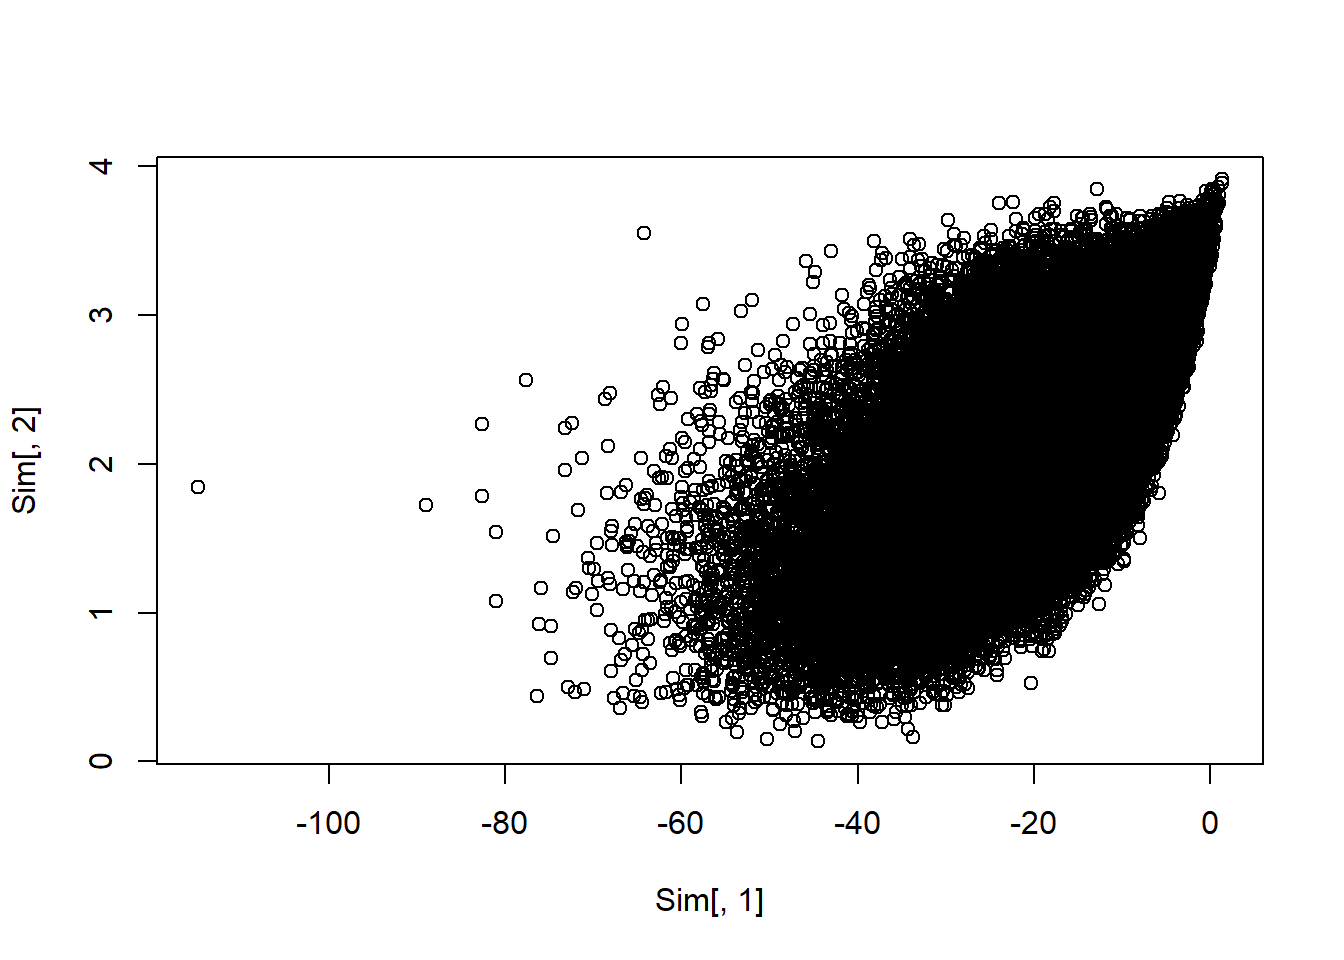
\includegraphics{WS_methylation_files/figure-latex/unnamed-chunk-5-1.pdf}

\hypertarget{computing-the-p-values}{%
\subsection{Computing the p-values}\label{computing-the-p-values}}

\begin{Shaded}
\begin{Highlighting}[]
\NormalTok{lambda <-}\StringTok{ }\KeywordTok{Search_lambda}\NormalTok{(Sim,}\DataTypeTok{plot=}\OtherTok{TRUE}\NormalTok{)}
\end{Highlighting}
\end{Shaded}

\begin{verbatim}
## [1] "Rought search"
## [1] "Dichotomised search"
\end{verbatim}

\includegraphics{WS_methylation_files/figure-latex/unnamed-chunk-6-1.pdf}

\begin{Shaded}
\begin{Highlighting}[]
\NormalTok{Th <-}\StringTok{ }\NormalTok{Sim[,}\KeywordTok{c}\NormalTok{(}\StringTok{"L_h"}\NormalTok{)]}\OperatorTok{+}\NormalTok{lambda}\OperatorTok{*}\NormalTok{Sim[,}\KeywordTok{c}\NormalTok{(}\StringTok{"min_ph_pv"}\NormalTok{)]}
\NormalTok{muv <-}\StringTok{ }\KeywordTok{median}\NormalTok{(Th,}\DataTypeTok{na.rm =} \OtherTok{TRUE}\NormalTok{)}
\NormalTok{sdv <-}\StringTok{ }\KeywordTok{mad}\NormalTok{(Th,}\DataTypeTok{na.rm =} \OtherTok{TRUE}\NormalTok{)}
\CommentTok{####################################}
\CommentTok{##Test Value of the loci to be tested}
\CommentTok{####################################}
\NormalTok{th <-}\StringTok{  }\NormalTok{res[,}\DecValTok{1}\NormalTok{]}\OperatorTok{+}\NormalTok{lambda}\OperatorTok{*}\NormalTok{res[,}\DecValTok{2}\NormalTok{]}

\NormalTok{dat <-}\StringTok{ }\KeywordTok{data.frame}\NormalTok{(}\DataTypeTok{dens =} \KeywordTok{c}\NormalTok{(}\KeywordTok{c}\NormalTok{(th),}\KeywordTok{c}\NormalTok{(Th))}
\NormalTok{                  , }\DataTypeTok{lines =} \KeywordTok{c}\NormalTok{(}\KeywordTok{rep}\NormalTok{(}\StringTok{"obs"}\NormalTok{, }\KeywordTok{length}\NormalTok{(}\KeywordTok{c}\NormalTok{(th))), }\KeywordTok{rep}\NormalTok{( }\StringTok{"sim"}\NormalTok{, }\KeywordTok{length}\NormalTok{(}\KeywordTok{c}\NormalTok{(Th))) ))}
\CommentTok{#Plot.}
\KeywordTok{ggplot}\NormalTok{(dat, }\KeywordTok{aes}\NormalTok{(}\DataTypeTok{x =}\NormalTok{ dens, }\DataTypeTok{fill =}\NormalTok{ lines)) }\OperatorTok{+}\StringTok{ }\KeywordTok{geom_density}\NormalTok{(}\DataTypeTok{alpha =} \FloatTok{0.5}\NormalTok{)}\OperatorTok{+}\KeywordTok{ggtitle}\NormalTok{(}\StringTok{"Test stat density"}\NormalTok{)}
\end{Highlighting}
\end{Shaded}

\includegraphics{WS_methylation_files/figure-latex/unnamed-chunk-6-2.pdf}

\begin{Shaded}
\begin{Highlighting}[]
\NormalTok{pv <-}\StringTok{ }\DecValTok{1}\OperatorTok{-}\KeywordTok{pnorm}\NormalTok{(th,}\DataTypeTok{mean=}\NormalTok{muv,}\DataTypeTok{sd=}\NormalTok{sdv)}
\KeywordTok{hist}\NormalTok{(}\DecValTok{1}\OperatorTok{-}\KeywordTok{pnorm}\NormalTok{(th,}\DataTypeTok{mean=}\NormalTok{muv,}\DataTypeTok{sd=}\NormalTok{sdv),}\DataTypeTok{nclass=}\DecValTok{100}\NormalTok{)}
\end{Highlighting}
\end{Shaded}

\includegraphics{WS_methylation_files/figure-latex/unnamed-chunk-7-1.pdf}

\begin{Shaded}
\begin{Highlighting}[]
\KeywordTok{hist}\NormalTok{(}\KeywordTok{log10}\NormalTok{(}\DecValTok{1}\OperatorTok{-}\KeywordTok{pnorm}\NormalTok{(th,}\DataTypeTok{mean=}\NormalTok{muv,}\DataTypeTok{sd=}\NormalTok{sdv)))}
\end{Highlighting}
\end{Shaded}

\includegraphics{WS_methylation_files/figure-latex/unnamed-chunk-7-2.pdf}

\hypertarget{loading-data-from-irizzary-et-al-2009-nature-genetics}{%
\subsection{Loading data from Irizzary et al 2009 Nature
Genetics}\label{loading-data-from-irizzary-et-al-2009-nature-genetics}}

\begin{Shaded}
\begin{Highlighting}[]
\KeywordTok{library}\NormalTok{(readxl)}
\NormalTok{tt <-}\StringTok{ }\KeywordTok{read_excel}\NormalTok{(}\StringTok{"D:/Document/Serieux/Travail/Data_analysis_and_papers/Fast functional association analysis based on wavelets/additionnal_simulation_AOAS/41588_2009_BFng298_MOESM18_ESM.xls"}\NormalTok{)}
\NormalTok{sub <-}\StringTok{ }\NormalTok{tt[}\KeywordTok{which}\NormalTok{(tt[,}\DecValTok{2}\NormalTok{]}\OperatorTok{==}\StringTok{"chr3"}\NormalTok{),]}
\NormalTok{sub <-}\StringTok{ }\KeywordTok{as.data.frame}\NormalTok{(sub}
\NormalTok{)}

\NormalTok{lstemp <-}\StringTok{ }\KeywordTok{list}\NormalTok{()}

\ControlFlowTok{for}\NormalTok{ (i }\ControlFlowTok{in} \DecValTok{1}\OperatorTok{:}\StringTok{ }\KeywordTok{dim}\NormalTok{(sub)[}\DecValTok{1}\NormalTok{])}
\NormalTok{\{}
  
\NormalTok{  lstemp[[i]] <-}\StringTok{ }\NormalTok{temp.pos[ }\KeywordTok{which}\NormalTok{( (sub}\OperatorTok{$}\NormalTok{start[i]}\OperatorTok{-}\DecValTok{1}\NormalTok{)  }\OperatorTok{<}\StringTok{ }\NormalTok{temp.pos }\OperatorTok{&}\StringTok{ }\NormalTok{temp.pos }\OperatorTok{<}\StringTok{ }\NormalTok{(sub}\OperatorTok{$}\NormalTok{end[i] }\OperatorTok{+}\DecValTok{1}\NormalTok{ ))]}
  
\NormalTok{\}}

\KeywordTok{sum}\NormalTok{( }\KeywordTok{lengths}\NormalTok{(lstemp)) }\CommentTok{# the list referred by Lee and Morris}
\end{Highlighting}
\end{Shaded}

\begin{verbatim}
## [1] 1901
\end{verbatim}

\begin{Shaded}
\begin{Highlighting}[]
\NormalTok{pos_to_detect <-}\StringTok{  }\KeywordTok{do.call}\NormalTok{( c,lstemp)}\CommentTok{#List of the CpG to detect}
\end{Highlighting}
\end{Shaded}

\hypertarget{performing-a-slicing}{%
\subsection{Performing a slicing}\label{performing-a-slicing}}

Ensure same slicing than before

\begin{Shaded}
\begin{Highlighting}[]
\NormalTok{thresh <-}\StringTok{ }\DecValTok{500}

\NormalTok{tl <-}\StringTok{ }\KeywordTok{split}\NormalTok{(temp.pos , }\KeywordTok{cumsum}\NormalTok{(}\KeywordTok{c}\NormalTok{(}\DecValTok{1}\NormalTok{, }\KeywordTok{diff}\NormalTok{(temp.pos) }\OperatorTok{>}\StringTok{ }\NormalTok{thresh)  ) ) }\CommentTok{#Remove case with too long distance}
\NormalTok{tl <-}\StringTok{  }\NormalTok{tl[}\OperatorTok{-}\KeywordTok{which}\NormalTok{(}\KeywordTok{lengths}\NormalTok{(tl) }\OperatorTok{<}\DecValTok{17}\NormalTok{)]}\CommentTok{#Keep only long enough sequence of CPG}

\NormalTok{pos_to_detect <-}\StringTok{ }\NormalTok{pos_to_detect [}\KeywordTok{which}\NormalTok{(pos_to_detect }\OperatorTok\StringTok{ }\KeywordTok{do.call}\NormalTok{( c , tl))] }\CommentTok{#filtering out the CpG remove when slicing}
\end{Highlighting}
\end{Shaded}

\hypertarget{power-the-if-a-region-contains-more-than-one-cpg-that-is-differentially-methylated-then-it-has-to-be-deteceted}{%
\subsection{Power the if a region contains more than one CpG that is
differentially methylated then it has to be
deteceted}\label{power-the-if-a-region-contains-more-than-one-cpg-that-is-differentially-methylated-then-it-has-to-be-deteceted}}

\begin{Shaded}
\begin{Highlighting}[]
\CommentTok{#N° of CpG per regions}
\NormalTok{n_CpG_per_region <-}\StringTok{ }\KeywordTok{list}\NormalTok{()}




\ControlFlowTok{for}\NormalTok{ ( i }\ControlFlowTok{in} \DecValTok{1}\OperatorTok{:}\KeywordTok{length}\NormalTok{(tl))}
\NormalTok{\{}
\NormalTok{  n_CpG_per_region[[i]] <-}\StringTok{ }\NormalTok{pos_to_detect[}\KeywordTok{which}\NormalTok{(pos_to_detect }\OperatorTok\StringTok{ }\NormalTok{tl[[i]])]}

\NormalTok{\}}


\NormalTok{nCpG_reg <-}\StringTok{ }\KeywordTok{lengths}\NormalTok{(n_CpG_per_region)}
\NormalTok{indx_to_detect <-}\StringTok{ }\KeywordTok{which}\NormalTok{( nCpG_reg }\OperatorTok{>}\DecValTok{0}\NormalTok{)}
\NormalTok{indx_to_detect}
\end{Highlighting}
\end{Shaded}

\begin{verbatim}
##  [1]    4    5   14   18   21   56   58   80  100  120  130  134  139  140  143
## [16]  157  168  189  190  221  232  249  327  337  375  413  416  417  448  479
## [31]  508  520  521  527  587  610  614  642  647  670  676  677  689  725  731
## [46]  741  748  760  771  774  775  777  778  795  801  803  804  806  814  817
## [61]  821  822  832  849  858  859  878  879  900  914  915  935  939  941  947
## [76]  977  995  997 1007 1008 1014 1019 1020 1021 1022 1024 1025 1045 1066
\end{verbatim}

When using p-values 10\^{}-5

\begin{Shaded}
\begin{Highlighting}[]
\NormalTok{indx_WS <-}\StringTok{  }\KeywordTok{which}\NormalTok{(pv }\OperatorTok{<}\StringTok{ }\DecValTok{10}\OperatorTok{^}\NormalTok{(}\OperatorTok{-}\DecValTok{5}\NormalTok{))}
\KeywordTok{length}\NormalTok{(indx_WS)}
\end{Highlighting}
\end{Shaded}

\begin{verbatim}
## [1] 76
\end{verbatim}

\begin{Shaded}
\begin{Highlighting}[]
\KeywordTok{sum}\NormalTok{(  indx_WS }\OperatorTok\StringTok{ }\NormalTok{indx_to_detect)}
\end{Highlighting}
\end{Shaded}

\begin{verbatim}
## [1] 76
\end{verbatim}

\begin{Shaded}
\begin{Highlighting}[]
\KeywordTok{which}\NormalTok{(indx_WS }\OperatorTok\StringTok{ }\NormalTok{indx_to_detect)}
\end{Highlighting}
\end{Shaded}

\begin{verbatim}
##  [1]  1  2  3  4  5  6  7  8  9 10 11 12 13 14 15 16 17 18 19 20 21 22 23 24 25
## [26] 26 27 28 29 30 31 32 33 34 35 36 37 38 39 40 41 42 43 44 45 46 47 48 49 50
## [51] 51 52 53 54 55 56 57 58 59 60 61 62 63 64 65 66 67 68 69 70 71 72 73 74 75
## [76] 76
\end{verbatim}

When using p-values 10\^{}-6

\begin{Shaded}
\begin{Highlighting}[]
\NormalTok{indx_WS <-}\StringTok{  }\KeywordTok{which}\NormalTok{(pv }\OperatorTok{<}\StringTok{ }\DecValTok{10}\OperatorTok{^}\NormalTok{(}\OperatorTok{-}\DecValTok{6}\NormalTok{))}
\KeywordTok{length}\NormalTok{(indx_WS)}
\end{Highlighting}
\end{Shaded}

\begin{verbatim}
## [1] 69
\end{verbatim}

\begin{Shaded}
\begin{Highlighting}[]
\KeywordTok{sum}\NormalTok{(  indx_WS }\OperatorTok\StringTok{ }\NormalTok{indx_to_detect)}
\end{Highlighting}
\end{Shaded}

\begin{verbatim}
## [1] 69
\end{verbatim}

\begin{Shaded}
\begin{Highlighting}[]
\KeywordTok{which}\NormalTok{(indx_WS }\OperatorTok\StringTok{ }\NormalTok{indx_to_detect)}
\end{Highlighting}
\end{Shaded}

\begin{verbatim}
##  [1]  1  2  3  4  5  6  7  8  9 10 11 12 13 14 15 16 17 18 19 20 21 22 23 24 25
## [26] 26 27 28 29 30 31 32 33 34 35 36 37 38 39 40 41 42 43 44 45 46 47 48 49 50
## [51] 51 52 53 54 55 56 57 58 59 60 61 62 63 64 65 66 67 68 69
\end{verbatim}

When using FDR

\begin{Shaded}
\begin{Highlighting}[]
\NormalTok{fdr_regions <-}\StringTok{ }\KeywordTok{p.adjust}\NormalTok{(pv, }\DataTypeTok{method =}\StringTok{"BH"}\NormalTok{)}
\NormalTok{indx_WS <-}\StringTok{  }\KeywordTok{which}\NormalTok{(fdr_regions  }\OperatorTok{<}\FloatTok{0.05}\NormalTok{)}
\KeywordTok{length}\NormalTok{(indx_WS)}
\end{Highlighting}
\end{Shaded}

\begin{verbatim}
## [1] 91
\end{verbatim}

\begin{Shaded}
\begin{Highlighting}[]
\KeywordTok{which}\NormalTok{(indx_WS }\OperatorTok\StringTok{ }\NormalTok{indx_to_detect)}
\end{Highlighting}
\end{Shaded}

\begin{verbatim}
##  [1]  1  2  3  4  5  6  7  9 10 11 12 13 14 15 16 17 18 19 20 21 22 23 24 25 26
## [26] 27 28 29 30 31 32 33 34 35 36 37 38 39 40 41 42 43 44 45 46 47 48 49 50 51
## [51] 52 53 54 55 56 57 58 59 60 61 62 63 64 65 66 67 68 69 70 71 72 73 74 75 76
## [76] 77 78 79 80 81 82 83 84 85 86 87 88 89 91
\end{verbatim}

\begin{Shaded}
\begin{Highlighting}[]
\KeywordTok{sum}\NormalTok{(  indx_WS }\OperatorTok\StringTok{ }\NormalTok{indx_to_detect)}
\end{Highlighting}
\end{Shaded}

\begin{verbatim}
## [1] 89
\end{verbatim}

\begin{Shaded}
\begin{Highlighting}[]
\NormalTok{fdr_regions <-}\StringTok{ }\KeywordTok{p.adjust}\NormalTok{(pv, }\DataTypeTok{method =}\StringTok{"BH"}\NormalTok{)}
\NormalTok{indx_WS <-}\StringTok{  }\KeywordTok{which}\NormalTok{(fdr_regions  }\OperatorTok{<}\FloatTok{0.01}\NormalTok{)}
\KeywordTok{length}\NormalTok{(indx_WS)}
\end{Highlighting}
\end{Shaded}

\begin{verbatim}
## [1] 88
\end{verbatim}

\begin{Shaded}
\begin{Highlighting}[]
\KeywordTok{which}\NormalTok{(indx_WS }\OperatorTok\StringTok{ }\NormalTok{indx_to_detect)}
\end{Highlighting}
\end{Shaded}

\begin{verbatim}
##  [1]  1  2  3  4  5  6  8  9 10 11 12 13 14 15 16 17 18 19 20 21 22 23 24 25 26
## [26] 27 28 29 30 31 32 33 34 35 36 37 38 39 40 41 42 43 44 45 46 47 48 49 50 51
## [51] 52 53 54 55 56 57 58 59 60 61 62 63 64 65 66 67 68 69 70 71 72 73 74 75 76
## [76] 77 78 79 80 81 82 83 84 85 86 88
\end{verbatim}

\begin{Shaded}
\begin{Highlighting}[]
\KeywordTok{sum}\NormalTok{(  indx_WS }\OperatorTok\StringTok{ }\NormalTok{indx_to_detect)}
\end{Highlighting}
\end{Shaded}

\begin{verbatim}
## [1] 86
\end{verbatim}

\end{document}
